\documentclass{article}
\usepackage[utf8]{inputenc}
\usepackage{parskip}
\usepackage{amsmath}
\usepackage{amssymb}
\usepackage[thinc]{esdiff}
\usepackage{tikz}
\usetikzlibrary{calc}

\title{Bar on Rollers - Dynamics Problem}

\author{
    Yip, Henry\\
    s2231321@ed.ac.uk
    \and
    Richmond, Lorian\\
    s2188785@ed.ac.uk
}

\date{March 2022}

\begin{document}

\maketitle

\section{The Problem}

A uniform bar of mass $m$ rests on two rollers, $r_1$ and $r_2$, separated by distance $d$. The rollers are rapidly rotating in opposite directions as shown in Fig \ref{problem_diagram}, and the coefficient of kinetic friction between the rollers and the bar is $\mu_k$.

$x$ is defined as the distance between $r_1$ and the centre of mass of the bar, $C$. When $t=0$, $x=x_0$ and $\dot{x}=0$.

Find $x$ as a function of time. How does the answer change if both rollers reverse their direction of rotation?

\begin{center}
	\label{problem_diagram}
	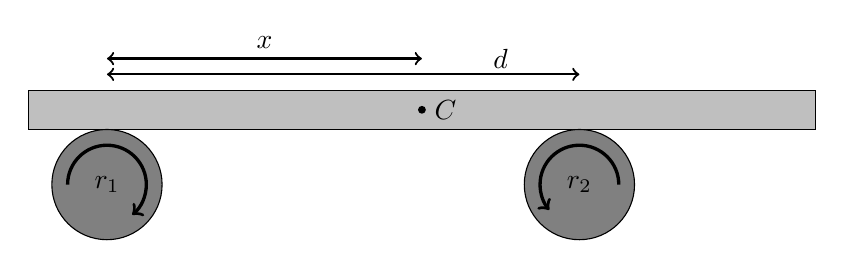
\begin{tikzpicture}
	    \filldraw[color=black, fill=lightgray] (0,0.7) rectangle ++(10,0.5);
	    \filldraw[color=black, fill=gray](1,0) circle (0.7);
	    \filldraw[color=black, fill=gray](7,0) circle (0.7);
	    \draw[draw=black, very thick, ->] (0.5,0) arc (180:-50:0.5);
	    \draw[draw=black, very thick, ->] (7.5,0) arc (0:220:0.5);
	    \draw[draw=black, thick, <->] (1,1.6) -- (5,1.6);
	    \draw[draw=black, thick, <->] (1,1.4) -- (7,1.4);
	    \node at (1,0) {$r_1$};
	    \node at (7,0) {$r_2$};
	    \node at (3,1.8) {$x$};
	    \node at (6,1.6) {$d$};
	    \node at (5, 0.95)[circle,fill,inner sep=1pt]{};
	    \node at (5.3,0.95) {$C$};
	\end{tikzpicture}
\end{center}

\section{The Solution}
\subsection{Rollers rotating inwards}
Let $N_1$ and $N_2$ be the upward forces acting on the bar from $r_1$ and $r_2$ respectively. As the net vertical force is zero, we know that
\begin{equation}
    \label{zero_vertical_force}
    N_1 + N_2 = mg
\end{equation}
The bar only moves horizontally and does not rotate, so we know that the torque about $r_1$ (or rather, a point above $r_1$ also level with $C$) must be zero. The only forces which contribute to this torque are $N_2$ acting upwards at distance $d$, and $mg$ acting downwards at distance $x$. Therefore:
\begin{align}
    N_2d &= mgx\\
    \implies N_2 &= \frac{mgx}{d}
    \label{expression_for_N2}
\end{align}
Substituting into (\ref{zero_vertical_force}):
\begin{align}
    N_1 &= mg - N_2\\
    &= mg - \left[ \frac{mgx}{d} \right]\\
    &= \frac{mg}{d} \cdot (d-x)
    \label{expression_for_N1}
\end{align}
Let $T_1$ and $T_2$ be the horizontal forces on the bar from $r_1$ and $r_2$ respectively. The rollers are rotating rapidly, so we can assume that both are slipping - this means that the horizontal force on the bar from each roller is given by $\mu_kF_N$ where $F_N$ is the normal force between the roller and the bar. Substituting (\ref{expression_for_N2}) and (\ref{expression_for_N1}) yields:
\begin{align}
    T_1 &= \frac{mg\mu_k}{d} \cdot (d-x)\\
    T_2 &= \frac{mg\mu_k}{d} \cdot x
\end{align}
By inspection of the diagram, we can tell that $T_1$ is acting to the right and $T_2$ is acting to the left. We can sum them to find the total force on the bar:
\begin{align}
    F_x &= T_1 - T_2\\
    &= \left[ \frac{mg\mu_k}{d} \cdot (d-x) \right] - \left[ \frac{mg\mu_k}{d} \cdot x \right]\\
    &= \frac{mg\mu_k}{d} \cdot (d-2x)
\end{align}
Then apply Newton's second Law to find the acceleration:
\begin{align}
    \ddot{x} &= \frac{F_x}{m}\\
    &= \frac{\mu_kg}{d} (d-2x)\\
    &= -\frac{2\mu_kg}{d} \left[ x-\frac{d}{2} \right]
\end{align}
Notice that this equation describes simple harmonic motion (SHM) with angular frequency $\omega = \sqrt{\frac{2\mu_kg}{d}}$ about $x=\frac{d}{2}$. We can then substitute into the standard solution for SHM, and use the stated boundary conditions to determine the unknown constants $A$ and $B$.
\begin{equation}
    x = A sin(\omega t) + B cos(\omega t) + \frac{d}{2}
\end{equation}
\begin{align}
    x(0) &= x_0\\
    \implies B &= x_0 - \frac{d}{2}
\end{align}
\begin{align}
    \dot{x}(0) &= 0\\
    \implies \omega A cos(\omega t) - \omega B sin(\omega t) + \frac{d}{2} &= 0\\
    \implies A &= 0
\end{align}
So our expression for $x$ in terms of $t$ is just:
\begin{equation}
    x = \frac{d}{2} + \left[ x_0 - \frac{d}{2} \right] \cos \left( \sqrt{\frac{2\mu_kg}{d}} t \right)
\end{equation}

\subsection{Rollers rotating outwards}
When the rollers are rotating in the opposite direction, $F_x = T_2 - T_1$ rather than $T_1 - T_2$.
\begin{align}
    F_x &= T_1 - T_2\\
    &= \left[ \frac{mg\mu_k}{d} \cdot x \right] - \left[ \frac{mg\mu_k}{d} \cdot (d-x) \right]\\
    &= \frac{mg\mu_k}{d} \cdot (2x-d)
\end{align}
This time we find the acceleration to be
\begin{equation}
    \ddot{x} = \frac{2\mu_kg}{d} \left[ x - \frac{d}{2} \right]
\end{equation}
Notice that this equation describes exponential growth or decay, and has the general solution\footnote{See \bf{Appendix A} for a rigorous proof}
\begin{equation}
    x - \frac{d}{2} = A e^{\lambda t} + B e^{-\lambda t} 
\end{equation}
Where $\lambda=\sqrt{\frac{2\mu_kg}{d}}$ and $A$ and $B$ are unknown constants. Using boundary conditions to solve for $A$ and $B$:
\begin{align}
    x(0) &= x_0\\
    \implies A + B &= x_0 - \frac{d}{2}\\
\end{align}
\begin{align}
    \dot{x}(0) &= 0\\
    \implies \lambda A e^{\lambda t} + \lambda B e^{-\lambda t} &= 0\\
    \implies A &= B
\end{align}
So our final expression for $x$ in terms of $t$ is:
\begin{align}
    x &= \frac{d}{2} + \frac{2x_0 - d}{4} \left[ e^{\sqrt{\frac{2\mu_kg}{d}} t} + e^{-\sqrt{\frac{2\mu_kg}{d}} t} \right]\\
    &= \frac{d}{2} + \left[ x_0 - \frac{d}{2} \right] \cosh \left( \sqrt{\frac{2\mu_kg}{d}} t \right)
\end{align}
Note that this is exactly the same solution as when the rollers are rotating inwards, except that $\cos$ is now $\cosh$. 
\section{Appendix A}

Consider the homogeneous equation:
\begin{equation}
\ddot{y}+ \alpha\dot{y}+ \beta y = 0
\end{equation}
By basic differentiation techniques, we have 
 \begin{align}
 \frac{d}{dx}(e^x)=e^x\\
 \implies \frac{d}{dx}(ae^x)=ae^x
 \end{align}
 
 Suppose that f: $\mathbb{R} \rightarrow \mathbb{R}$ is differentiable everywhere and $f'(x)=af(x)$.
 There are no other functions in which the derivative is equal to itself. 
 \subsection{Proof 1}

 If we let $g(x)=\frac{af(x)}{e^{ax}}$


$ f(x)$ and $e^{ax}$ are differentiable $\rightarrow g'(x)$ is defined.
\begin{align}
     g'(x)&=\frac{f'(x)e^{ax}-af(x)e^{ax}}{(e^{ax})^2}\\
     g'(x)&=\frac{af(x)e^{ax}-af(x)e^{ax}}{(e^{ax})^2}\\
     g'(x)&=0
\end{align}
 By identity theorem, $g'(x)=0\rightarrow g(x)= c$, where $c\in \mathbb{R}$\\
 \implies $f(x)=Ae^{ax}$, where $A=ac$. We take $a=1$ and hence $A=c$.
 The above statement can be proved by Picard–Lindelöf theorem, however we won't cover it here.
 \subsection{Proof 2}
 Suppose that f: $\mathbb{R} \rightarrow \mathbb{R}$ is differentiable everywhere and $f(x)=f'(x)$
 \begin{align}
     1&=\frac{f(x)}{f'(x)}\\
     x+c&=\int{\frac{f(x)}{f'(x)}}, c\in \mathbb{R}\\
     x+c&=ln(f(x))\\
     f(x)&=e^{x+c}\\
     f(x)&=\gamma e^x, \gamma =e^c
 \end{align}
 \subsection{Ansatz}
 Therefore, we take the Ansatz: $y=e^{\lambda x}$ and obtain:
 \begin{align}
 \alpha \ddot{y}+ \beta\dot{y}+ \gamma y &= 0\\
     ({\lambda}^2 + \alpha\lambda  + \beta)(e^{\lambda x}) &=0
\end{align}
     Obviously $e^{\lambda x}=0$ is undefined, so 
     \begin{equation}
     {\lambda}^2 + \alpha\lambda  + \beta=0
     \end{equation}
     \begin{equation}
     \lambda_1=\frac{a}{2}+\sqrt{\frac{a^2}{4}-b} 
     \end{equation}
     \begin{equation}
     \lambda_2=\frac{a}{2}-\sqrt{\frac{a^2}{4}-b}
     \end{equation}
     
     We can imagine both $\lambda_1$ and $\lambda_2$ satisfies the equation, so $y$ is a linear combination of $e^{\lambda_1 x}$ and $e^{\lambda_2 x}$, we can rewrite this as:
     \begin{equation}
         y=Ae^{\lambda_1 x}+Be^{\lambda_1 x}
     \end{equation}
     Where A \& B $\in \mathbb{R}$
     
     You can imagine $e^{\lambda_1 x}$ \& $e^{\lambda_2 x}$ being the basis vector in a 2-dimensional vector space. In other words, $y=A\bf{e^{\lambda_1 x}}+B\bf{e^{\lambda_2 x}}$ has only the trivial solution $A=B=0$ with  $e^{\lambda_1 x}$\& $e^{\lambda_2 x}$ being linearly independent. 
     
     Note that the above is only true for $\lambda_1 \ne \lambda_2$. For $\lambda_1 = \lambda_2$, it's a bit more abstract and will be written some other time.
 \end{document}

